\setcounter{section}{17}


\section{Lecture 18: March 1}


\subsection*{Last time}
\begin{itemize}
 \item Unusual and influential data (JF chapter 11)
\end{itemize}


\subsection*{Today}
\begin{itemize}
 \item HW2 deadline extends to end of this week.
 \item Diagnosing non-normality, non-constant error variance, and nonlinearity (JF chapter 12)
 \item Data transformation (JF chapter 4)
\end{itemize}


\subsubsection*{Central Limit Theorem}
Let $X_1, X_2, \dots$ be a sequence of iid random variables whose mgfs exist in a neighborhood of $0$ (that is, $M_{X_i}(t)$ exists for $|t| < h$, for some positive $h$).
Let $\mbox{E}{X_i}=\mu$ and $\sVar{X_i}=\sigma^2 >0$. (Both $\mu$ and $\sigma^2$ are finite since the mgf exists.). Define $\bar{X}_n = (1/n)\sum\limits_{i = 1}^n X_i$.
Let $G_n(x)$ denote the cdf of $\sqrt{n} (\bar{X}_n - \mu)/\sigma$.
Then, for any $x$, $-\infty < x < \infty$,
$$
\lim\limits_{n \to \infty} G_n(x) = \int_{-\infty}^x \frac{1}{\sqrt{2\pi}} e^{-y^2/2}dy
$$
that is, $\sqrt{n}(\bar{X}_n - \mu)/\sigma$ has a limiting standard normal distribution.
(Refer to Casella \& Berger p.237 - p.238 for a proof.)

\subsubsection*{Delta Method}
Let $Y_n$ be a sequence of random variables that satisfies $\sqrt{n} (Y_n - \theta) \to N(0, \sigma^2)$ in distribution.
For a given function $g$ and a specific value of $\theta$, suppose $g'(\theta)$ exists and is not $0$.  Then
$$
\sqrt{n} [ g(Y_n) - g(\theta) ] \to N(0, \sigma^2 [g'(\theta)]^2) \mbox{ in distribution}.
$$
(Refer to Casella \& Berger p.243 for a proof using Taylor expansion.)

\subsubsection*{Second-order Delta Method}
Let $Y_n$ be a sequence of random variables that satisfies $\sqrt{n} (Y_n - \theta) \to N(0, \sigma^2)$ in distribution.
For a given function $g$ and a specific value of $\theta$, suppose that $g'(\theta)=0$ and $g''(\theta)$ exists and is not $0$.  Then
$$
\sqrt{n} [ g(Y_n) - g(\theta) ] \to \sigma^2 \frac{g''(\theta)}{2} \chi_1^2  \mbox{ in distribution}.
$$

\subsection*{Non-normally distributed errors}

The assumption of normally distributed errors is almost always arbitrary.  
Nevertheless, the central limit theorem ensures that, under very broad conditions, inference based on the least-squares estimator is approximately valid in all but small samples.
Why concern about non-normal errors?
\begin{itemize}
  \item For some types of error distributions, particularly those with heavy tails, the efficiency of least-squares estimation decreases markedly.
  \item Highly skewed error distributions, aside from their propensity to generate outliers in the direction of the skew, compromise the interpretation of the least-squares fit.
  This fit is a conditional mean (of $Y$ given the $X$s), and the mean is not a good measure of the center of a highly skewed distribution.
  \item A multimodal error distribution suggests that omission of one or more discrete explanatory variables that divide the data naturally into groups.  
  An examination of the distribution of the residuals may motivate respecification of the model.
\end{itemize}

Note: The \underline{skewness $\alpha_3$} is defined as $\alpha_3 \equiv \frac{\mu_3}{(\mu_2)^{3/2}}$ where $\mu_n$ denotes the $n$th central moment of a random variable $X$.
The skewness measures the lack of symmetry in the pdf.

\subsubsection*{Quantile-comparison plot, JF 3.1.3}
{\it Quantile-comparison plots} are useful for comparing an empirical sample distribution with a theoretical distribution, such as the normal distribution.

Let $P(x)$ represent the theoretical cumulative distribution function (cdf) with which we want to compare the data, that is $P(x) = \Pr(X \le x)$.
The quantile-comparison plot is constructed by:
\begin{enumerate}
  \item Order the data values from smallest to largest, $X_{(1)}, X_{(2)}, \dots, X_{(n)}$.  The $X_{(i)}$ are called the \underline{order statistics} of the sample.
  \item By convention, the cumulative proportion of the data ``below'' $X_{(i)}$ is given by 
  $$
  P_i = \frac{i - \frac{1}{2}}{n}
  $$
  \item  Use the inverse of the cdf to find the value $z_i$ corresponding to the cumulative probability $P_i$, that is
  $$
  z_i = P^{-1}(\frac{i - \frac{1}{2}}{n})
  $$
  \item Plot the $z_i$ as horizontal coordinates against the $X_{(i)}$ as vertical coordinates.  If $X$ is sampled from the distribution $P$, then $X_{(i)}\approx z_i$.
  \begin{itemize}
    \item if the distributions are identical except for location, then the plot is approximately linear with nonzero intercept, $X_{(i)} \approx \mu + z_i$
    \item if the distributions are identical except for scale, then the plot is approximately linear with a slope different from $1$, $X_{(i)} \approx \sigma z_i$
    \item if the distributions differ both in location and scale but have the same shape, then $X_{(i)} \approx \mu + \sigma z_i$
  \end{itemize}
  \item It is often helpful to place a comparison line on the plot to facilitate the perception of departures from linearity.  
  For a normal quantile-comparison plot (comparing the distribution of the data with the standard normal distribution), we can alternatively use the median as a robust estimator of $\mu$ and the interquartile range/1.39 as a robust estimator of $\sigma$.
  \item We expect some departure from linearity because of sampling variation.
  It therefore assists interpretation to display the expected degree of sampling error in the plot.
  The standard error of the order statistic $X_{(i)}$ is 
  $$
  \mbox{SE}(X_{(i)}) = \frac{\hat{\sigma}}{p(z_i)} \sqrt{\frac{P_i(1 - P_i)}{n}}
  $$
  where $p(z_i)$ is the probability density function, pdf, corresponding to the CDF $P(z)$.
  The values along the fitted line are given by $\hat{X}_{(i)} = \hat{\mu} + \hat{\sigma}z_i$.
  An approximate 95\% confidence ``envelope'' around the fitted line is, therefore,
  $$
  \hat{X}_{(i)} \pm 2\times \mbox{SE}(X_{(i)}) 
  $$
\end{enumerate}

\begin{itemize}
  \item Figure~\ref{fig:JF_3_8} plots a sample of $n=100$ observations from a normal distribution with mean $\mu = 50$ and standard deviation $\sigma = 10$.
%
\begin{figure}[H]
	\begin{center}
		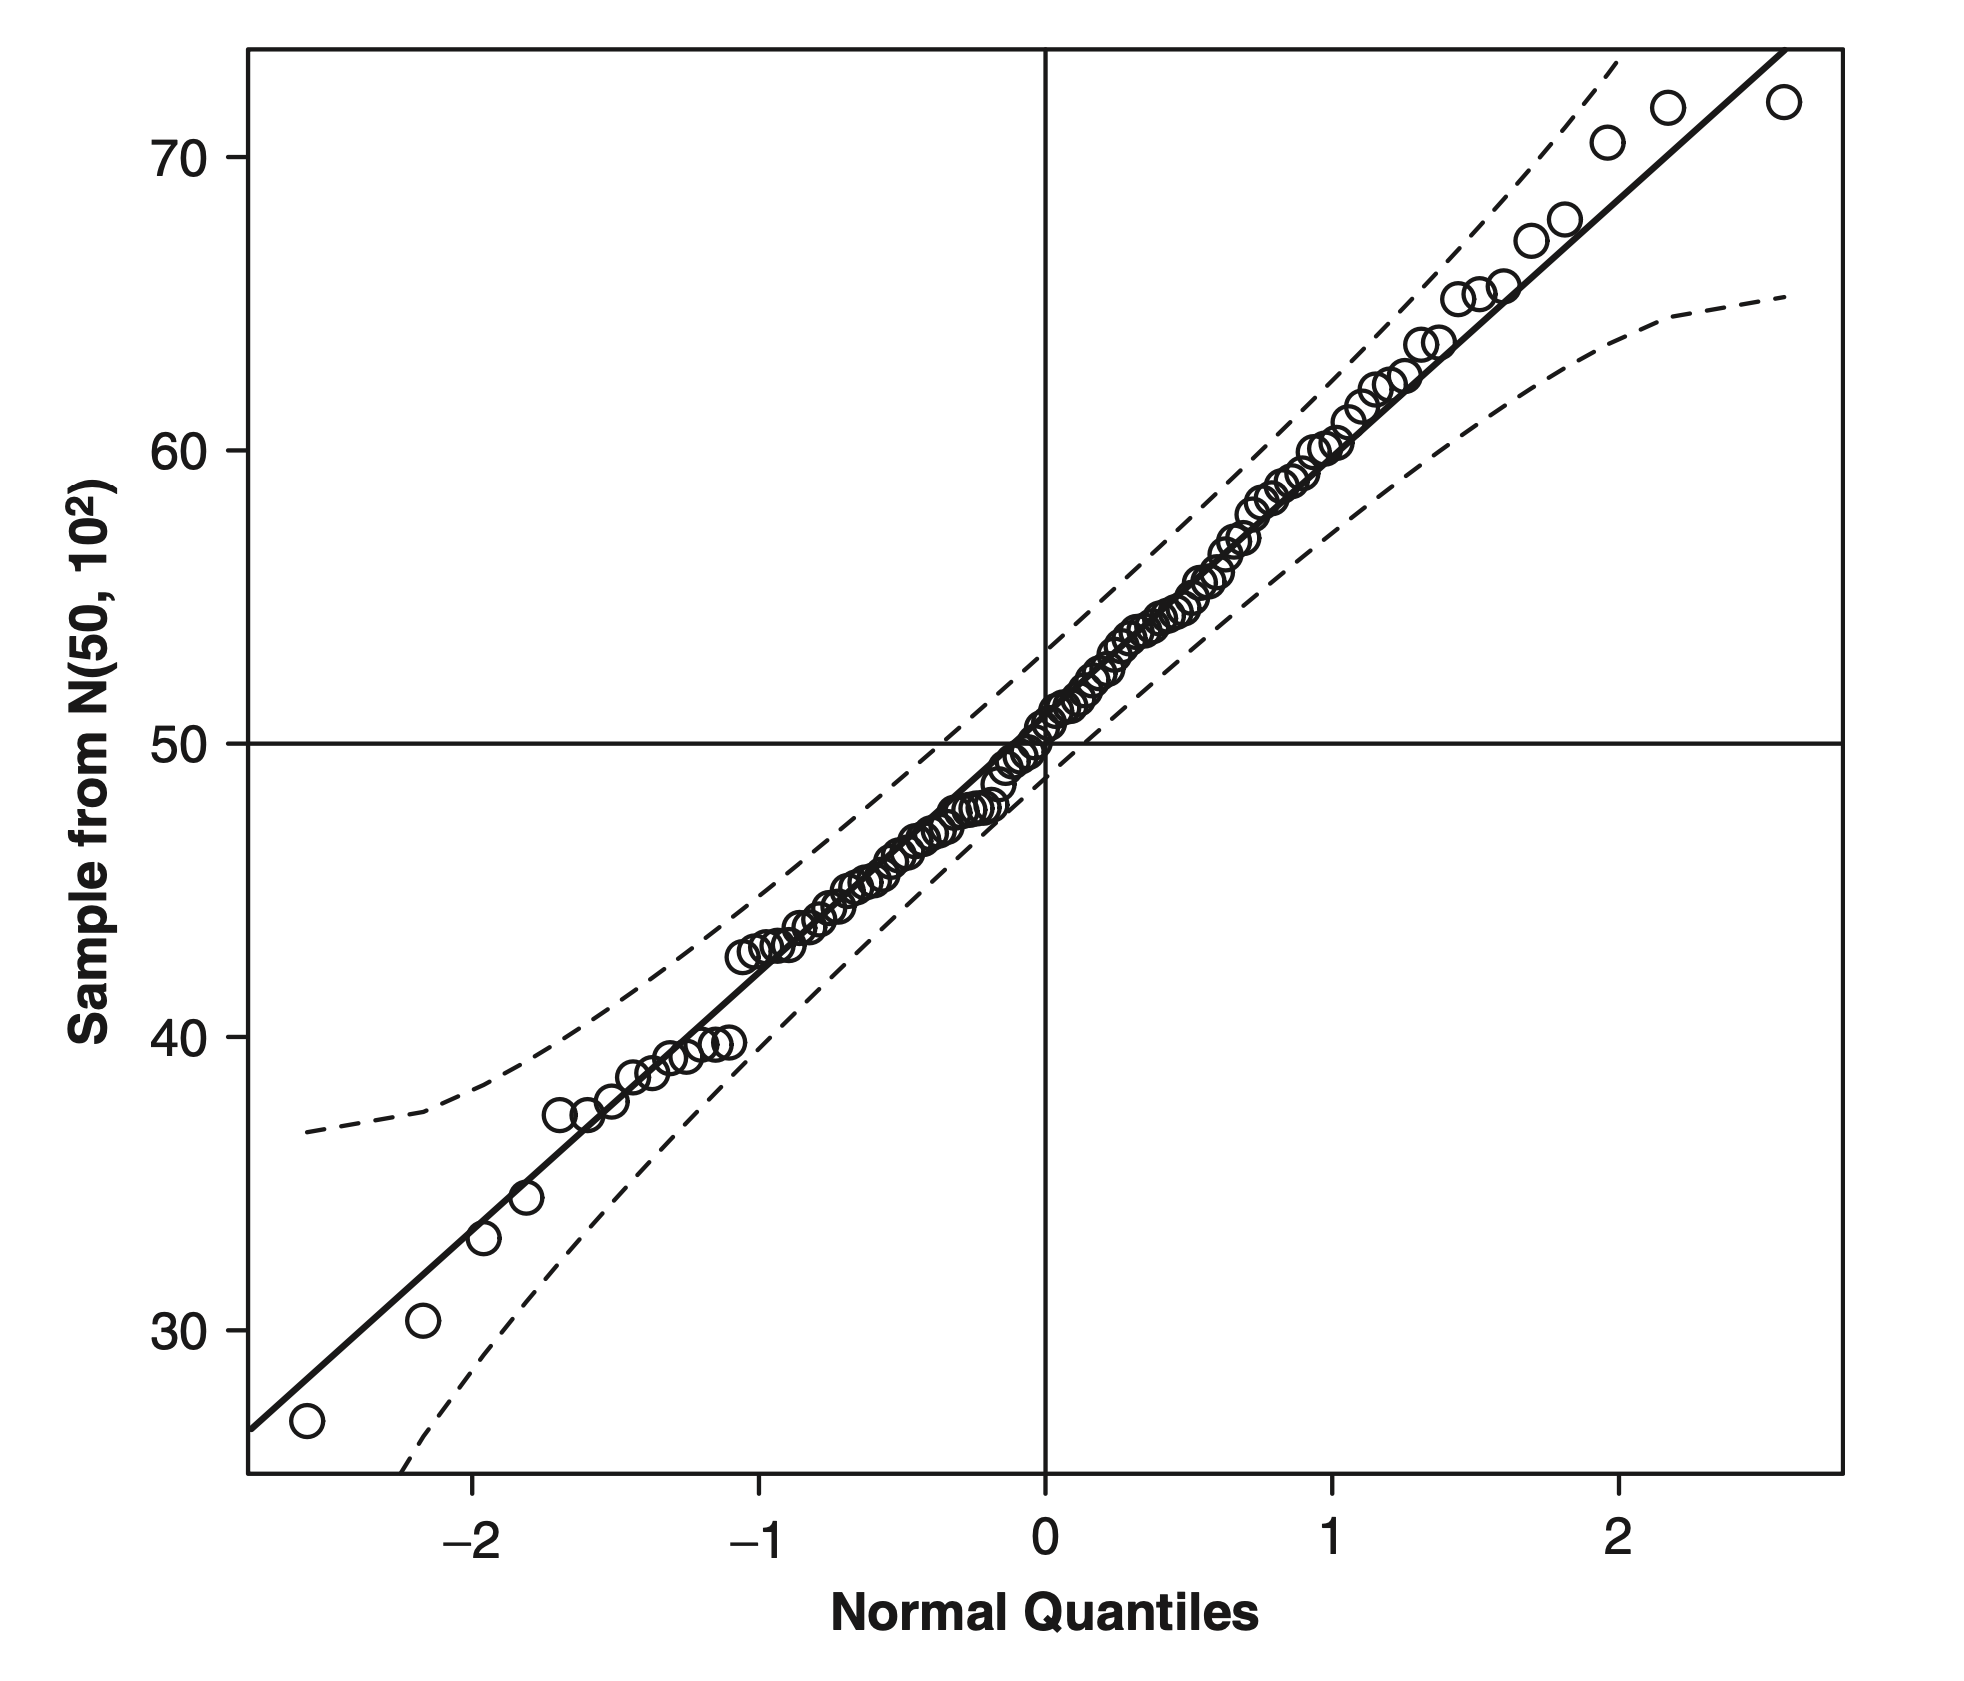
\includegraphics[width=0.8\textwidth]{Lecture18/JF_3_8}
		\caption{
			Normal quantile-comparison plot for a sample of $100$ observations drawn from a normal distribution with mean $50$ and standard deviation $10$.
			The fitted line is through the quartiles of the distribution, the broken lines give a pointwise 95\% confidence interval around the fit.
			JF Figure 3.8.}
		\label{fig:JF_3_8}
	\end{center}
\end{figure}
%  
  The plotted points are reasonably linear and stay within the rough 95\% confidence envelope.
  \item Figure~\ref{fig:JF_3_9} plots a sample of $n=100$ observations from the positively skewed chi-square distribution with 2 degrees of freedom.
  The positive skew of the data is reflected in points that lie {\it above} the comparison line in both tails of the distribution. (In contrast, the tails of negatively skewed data would lie {\it below} the comparison line.)
%
\begin{figure}[H]
	\begin{center}
		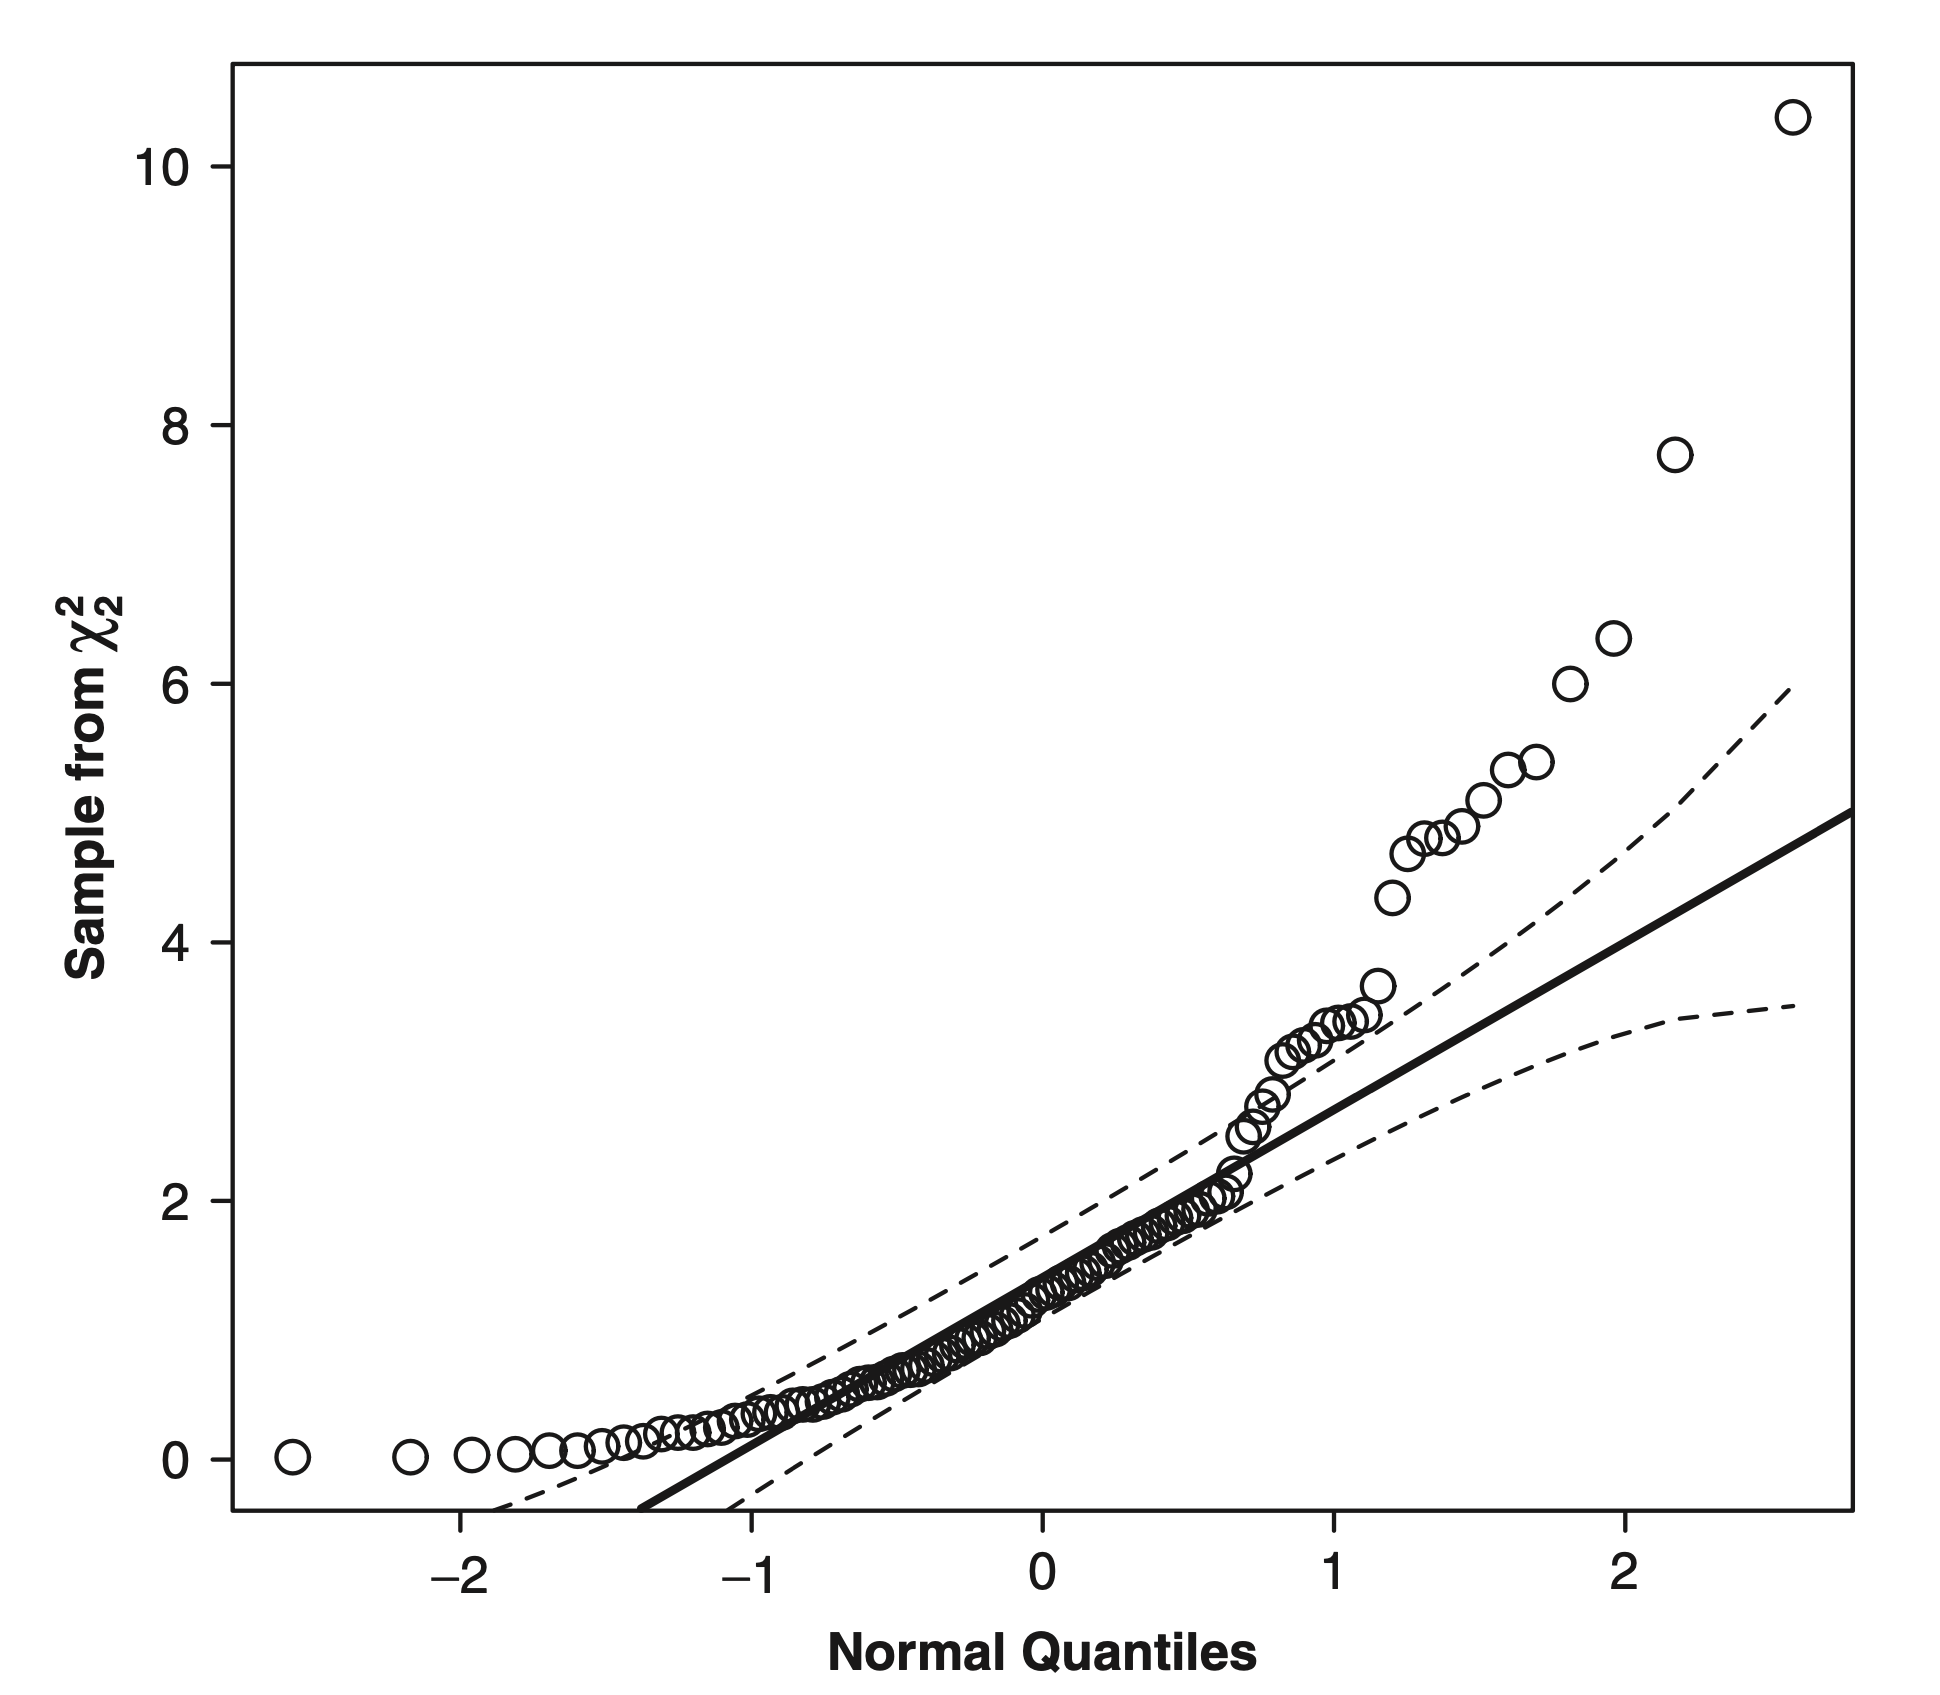
\includegraphics[width=0.8\textwidth]{Lecture18/JF_3_9}
		\caption{
			Normal quantile-comparison plot for a sample of $100$ observations drawn from the positively skewed chi-square distribution with 2 degrees of freedom.
			JF Figure 3.9.}
		\label{fig:JF_3_9}
	\end{center}
\end{figure}
%  
  \item Figure~\ref{fig:JF_3_10} plots a sample of $n = 100$ observations from the heavy-tailed $t$ distribution with 2 degrees of freedom.
  In this case, values in the upper tail lie above the corresponding normal quantiles, the values in the lower tail below the corresponding normal quantiles.
%
\begin{figure}[H]
	\begin{center}
		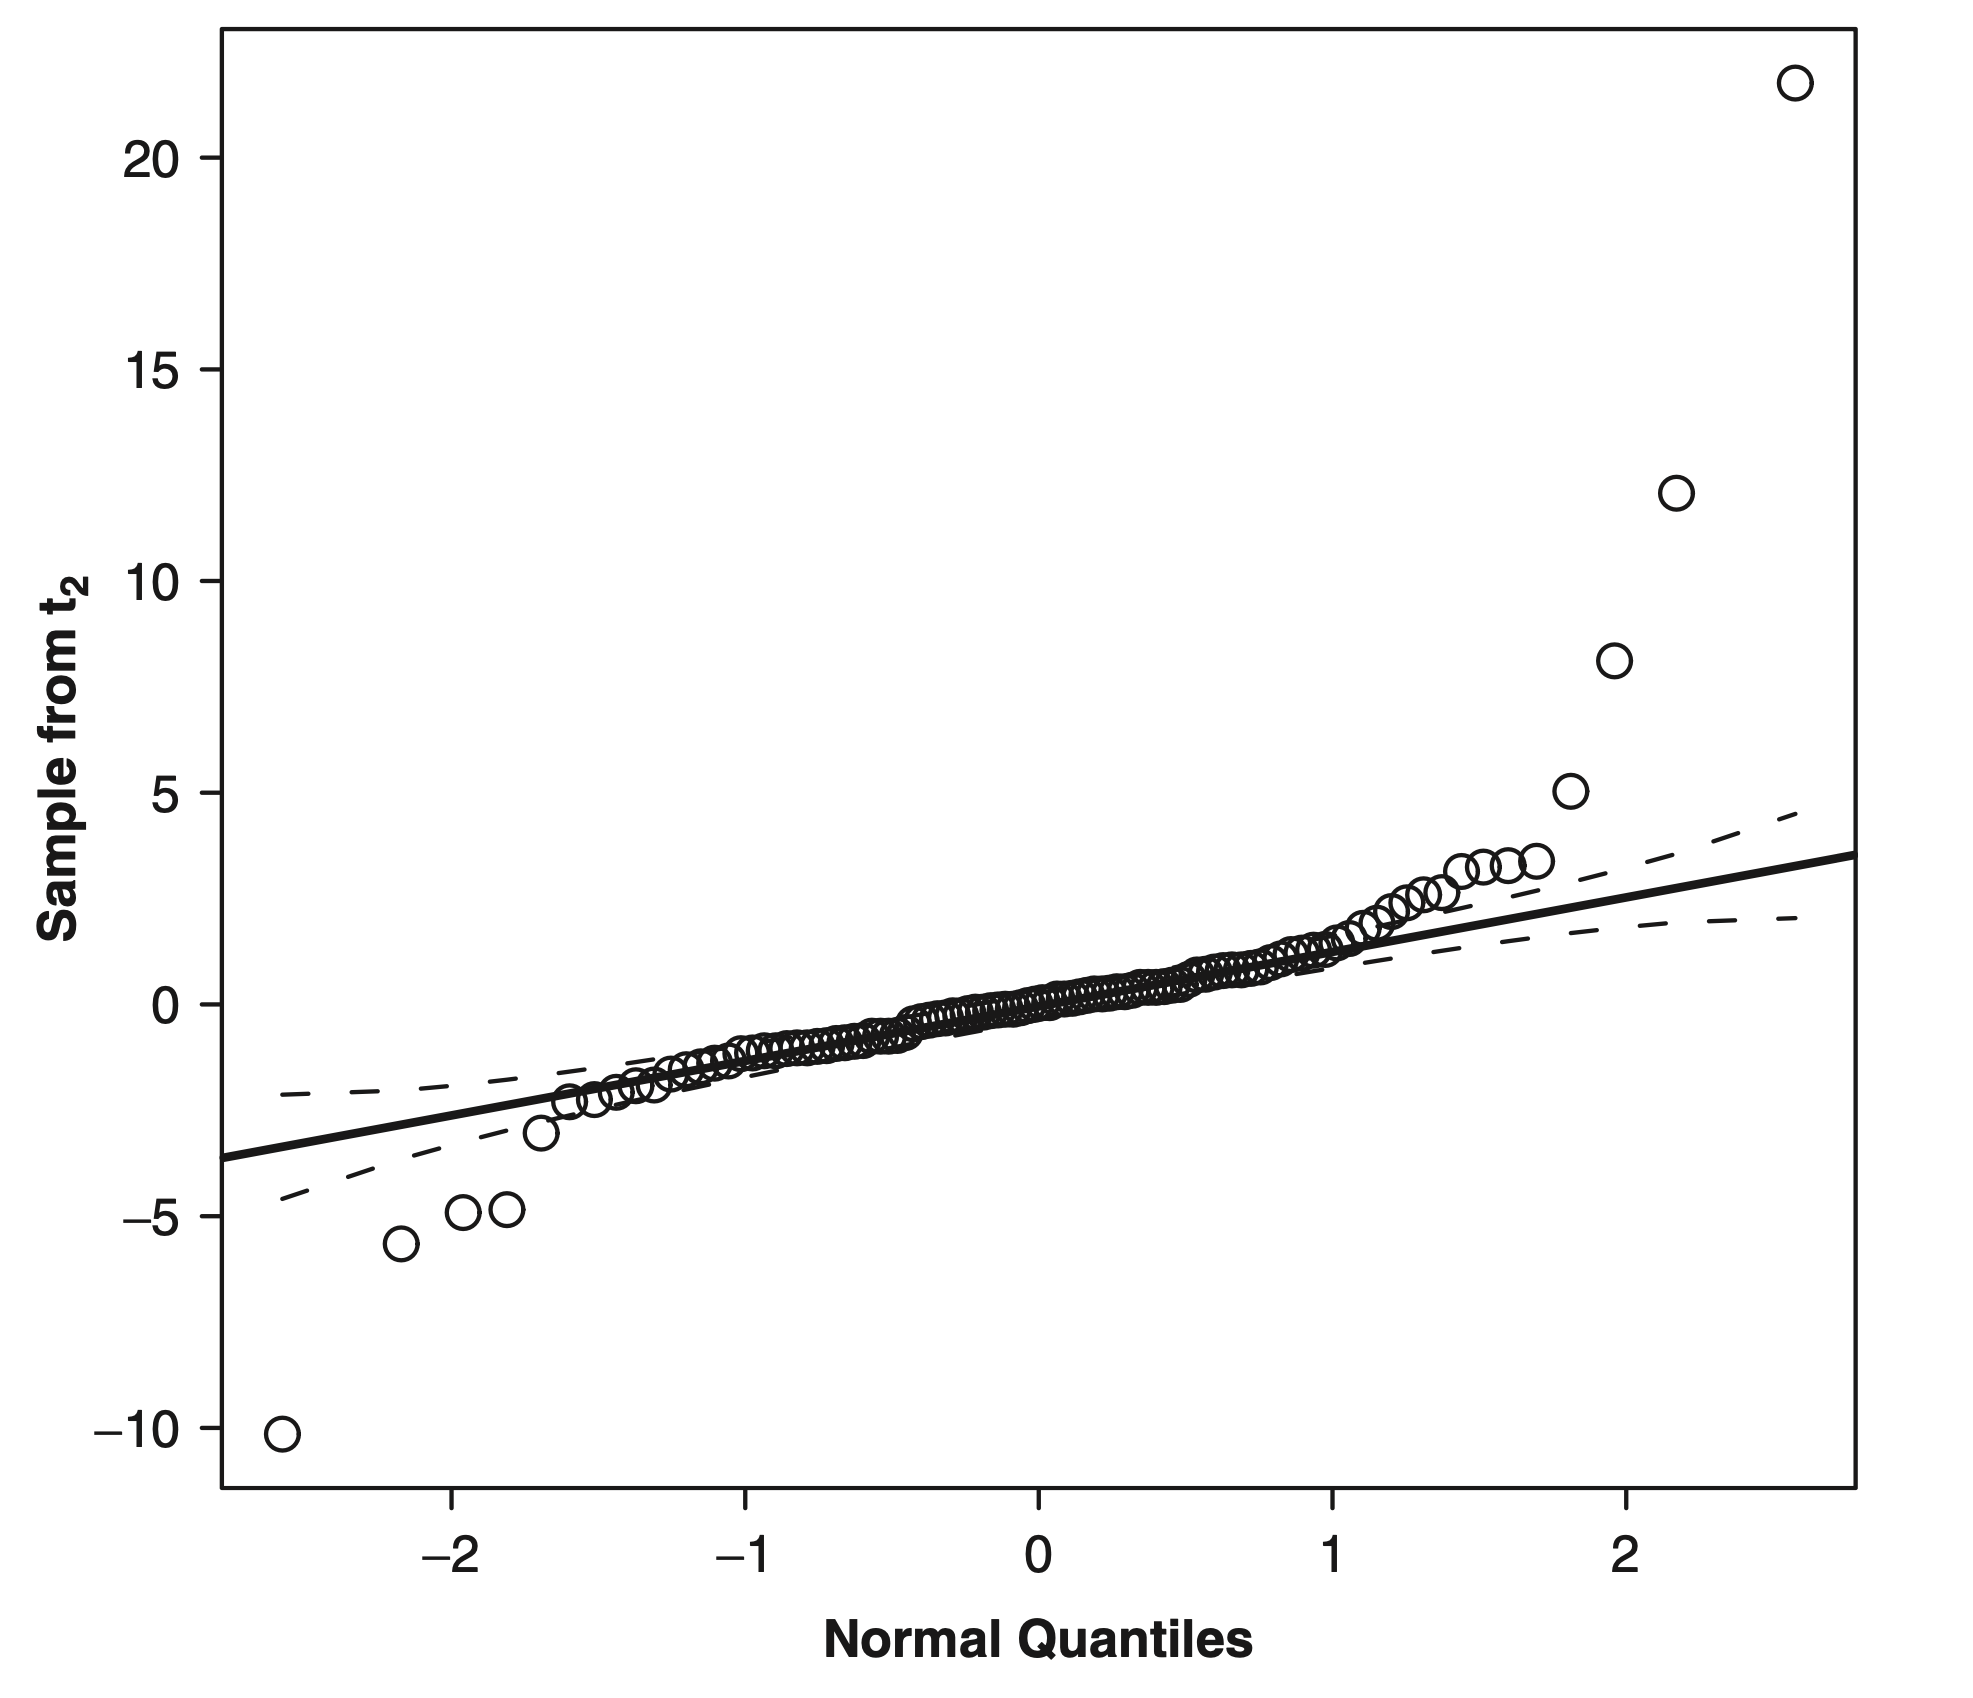
\includegraphics[width=0.8\textwidth]{Lecture18/JF_3_10}
		\caption{
			Normal quantile-comparison plot for a sample of $100$ observations drawn from heavy-tailed $t$-distribution with 2 degrees of freedom.
			JF Figure 3.10.}
		\label{fig:JF_3_10}
	\end{center}
\end{figure}
%  
  \item Figure~\ref{fig:JF_3_11} shows the normal quantile-comparison plot for the distribution of infant mortality.  The positive skew of the distribution is readily apparent.
%
\begin{figure}[H]
	\begin{center}
		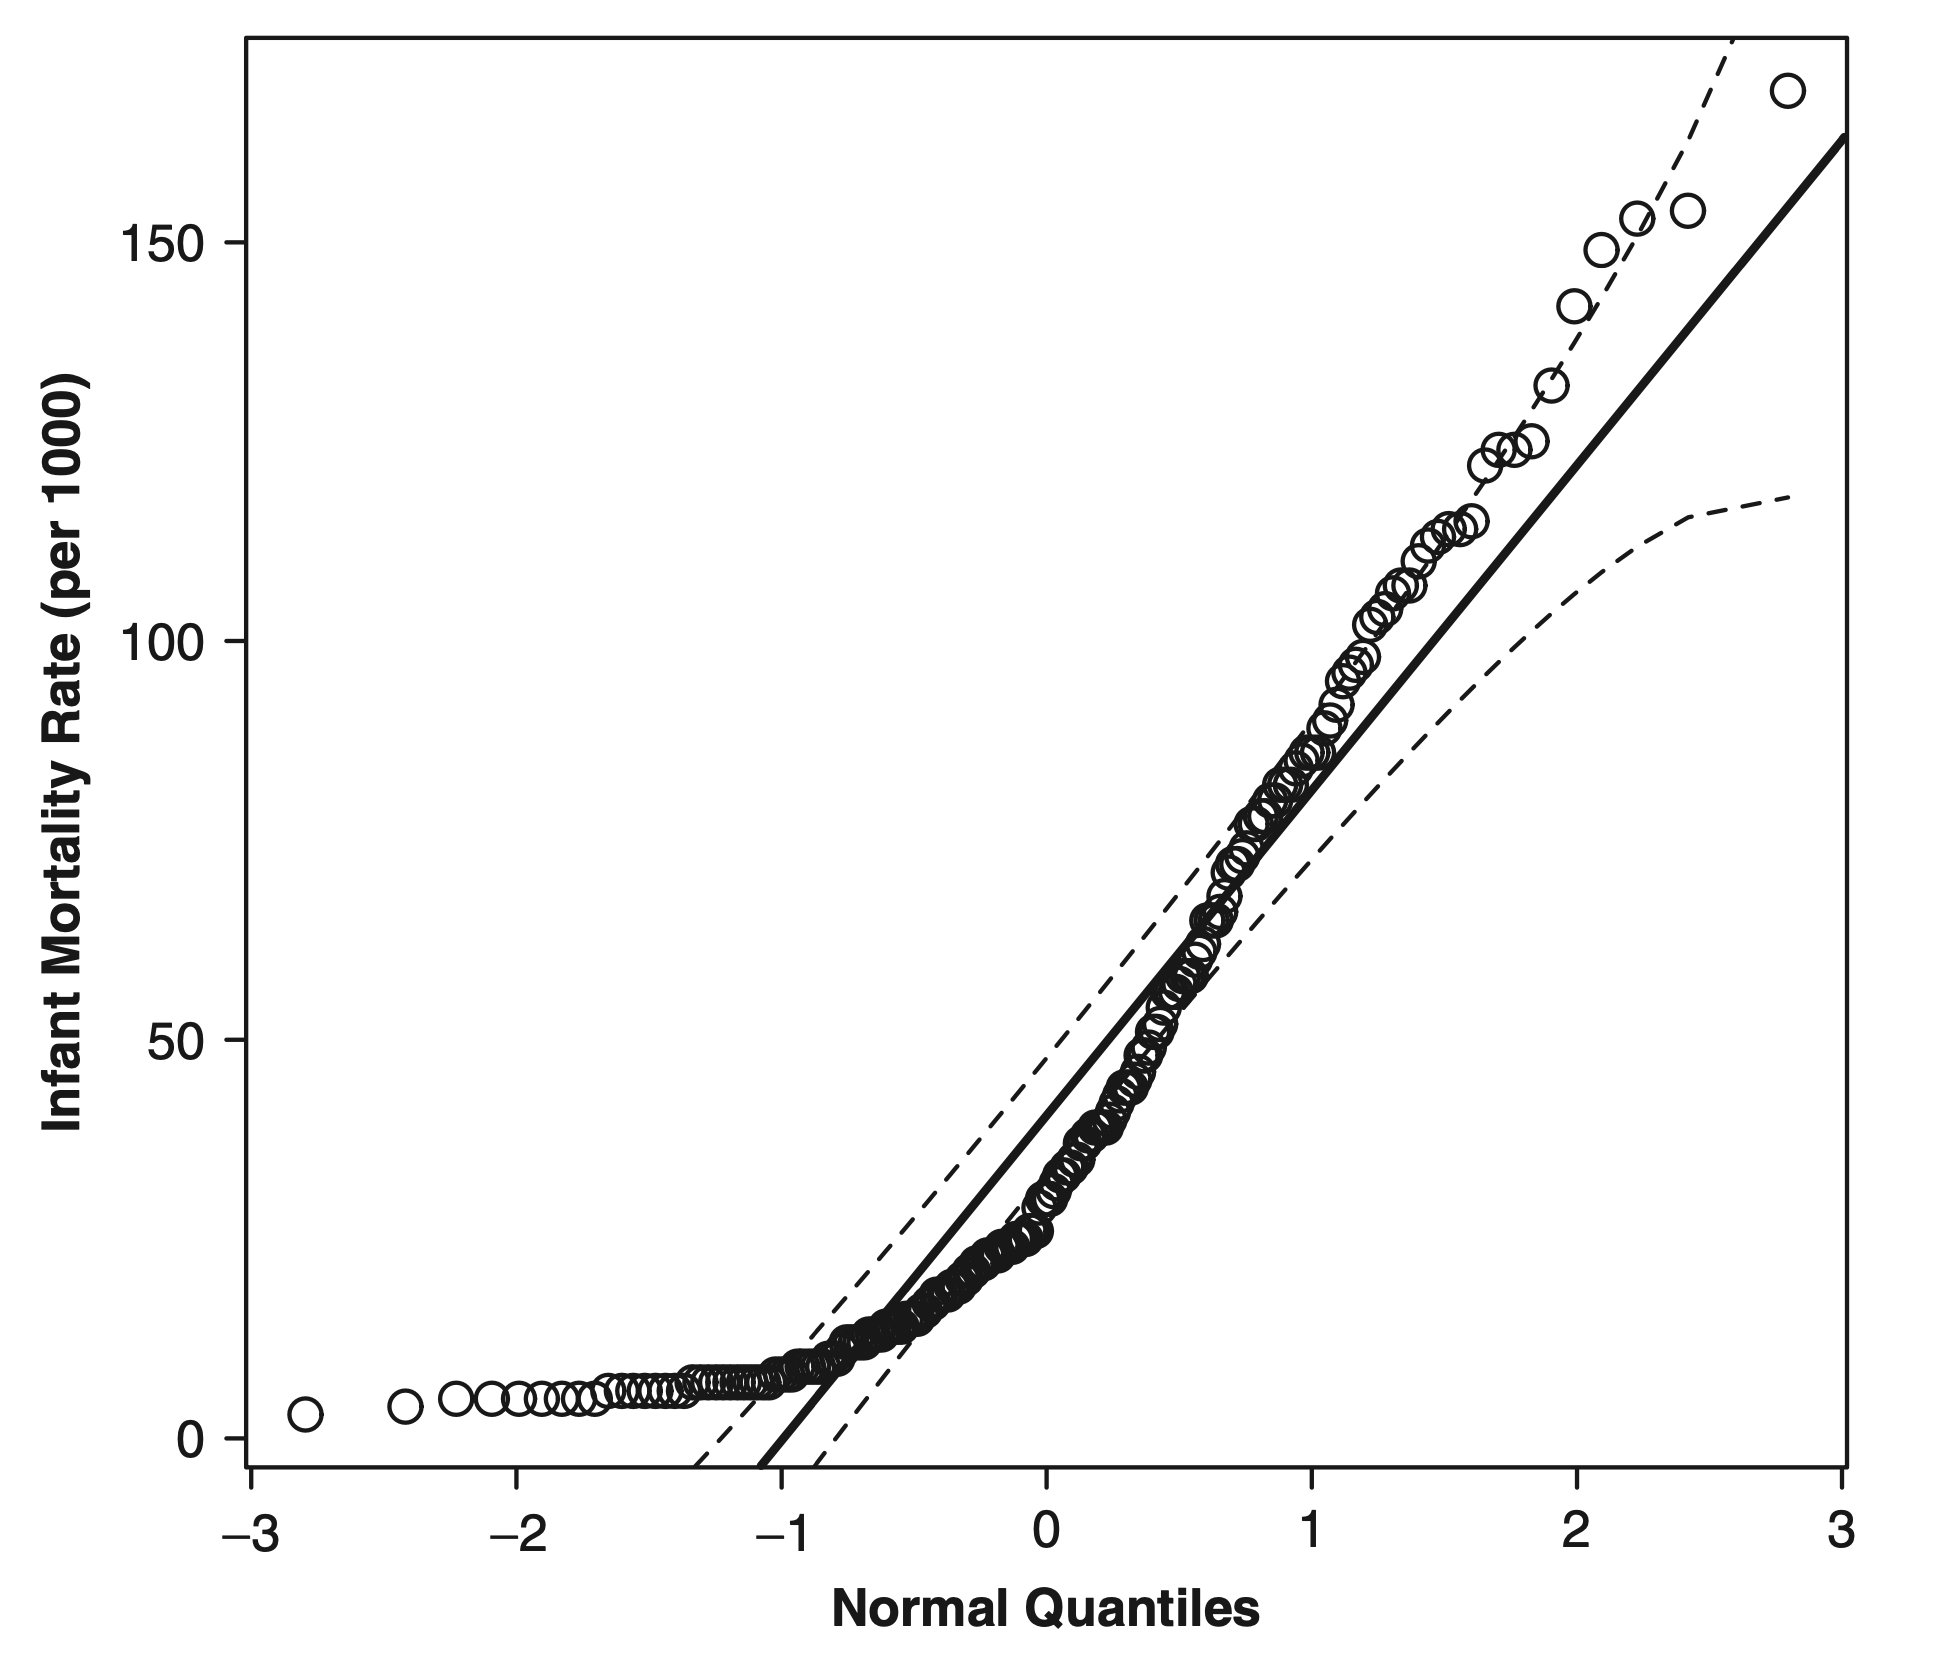
\includegraphics[width=0.8\textwidth]{Lecture18/JF_3_11}
		\caption{
			Normal quantile-comparison plot for the distribution of infant mortality.  Note the positive skew.
			JF Figure 3.11.}
		\label{fig:JF_3_11}
	\end{center}
\end{figure}
%  
\end{itemize}




\subsection*{Nonconstant error variance}
One of the assumptions of the regression model is that the variation of the response variable around the regression surface (the error variance) is everywhere the same:
$$
\sVar(\epsilon) = \sVar(Y | x_1, \dots, x_p) = \sigma_\epsilon^2
$$

Constant error variance is often termed \underline{homoscedasticity}, and similarly, nonconstant error variance is termed \underline{heteroscedasticity}.
We detect nonconstant error variances through graphical methods.

\subsubsection*{Residual plots}
Because the least square residuals have unequal variance even when the constant variance assumption is correct:
$$
\sVar(\hat{\epsilon}_i) = \sigma^2 (1 - h_i).
$$
It is preferable to plot studentized residuals against fitted values.
A pattern of changing spread is often more easily discerned in a plot of absolute studentized residuals, $|\hat{\epsilon}_i^{*}|$, or squared studentized residuals, $\hat{\epsilon}_i^{*2}$, against $\hat{Y}$.
If the values of $\hat{Y}$ are all positive, then we can plot $\log |\hat{\epsilon}_i^{*}|$ against $\log \hat{Y}$.
Figure~\ref{fig:JF_12_3} shows a plot of studentized residuals against fitted values and spread-level plot of studentized residuals, several points with negative fitted values were omitted.
%
\begin{figure}[H]
\begin{center}
  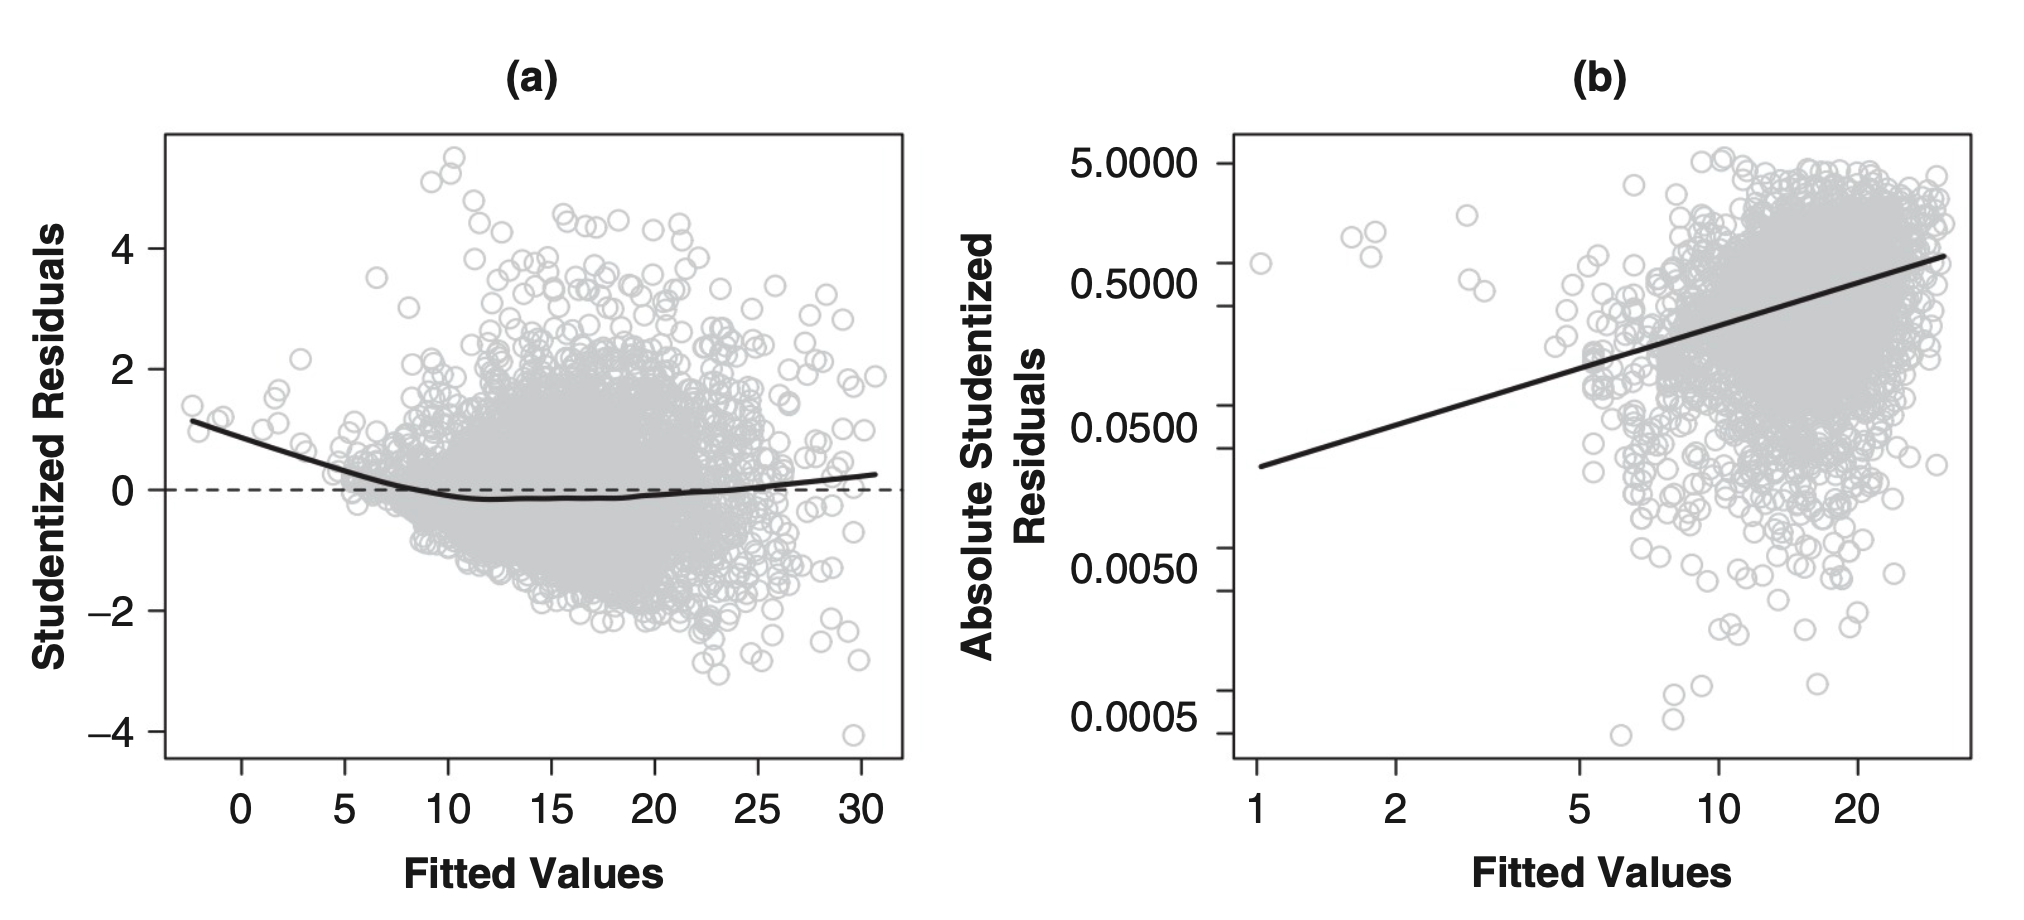
\includegraphics[width=0.9\textwidth]{Lecture18/JF_12_3}
  \caption{(a) Plot of studentized residuals versus fitted values and (b) spread-level plot for studentized residuals.
   JF Figure 12.3.}
  \label{fig:JF_12_3}
\end{center}
\end{figure}
%
It is apparent from both graphs that the residual spread tends to increase with the level of the response, suggesting a violation of constant error variance assumption.

\subsubsection*{Weighted-least-squares estimation}

\underline{Weighted-least-squares} (WLS) regression provides an alternative approach to estimation in the presence of nonconstant error variance.
Suppose that the errors from the linear regression model $\vecc{Y} = \vecc{X\beta} + \vecc{\epsilon}$ are independent and normally distributed, with zero means but {\it different} variances:
$\epsilon_i \sim N(0, \sigma^2_i)$.
Suppose further that the variances of the errors are known up to a constant of proportionality $\sigma_\epsilon^2$, so that $\sigma_i^2 = \sigma_\epsilon^2/w_i^2$.
Then the likelihood for the model is
$$
L(\beta, \sigma_\epsilon^2) = \frac{1}{(2\pi)^{n/2} |\vecc{\Sigma|}^{1/2}}\exp\left[ -\frac{1}{2}(\vecc{Y} - \vecc{X\beta})\transpose \vecc{\Sigma}^{-1} (\vecc{Y} - \vecc{X\beta}) \right]
$$
where $\vecc{\Sigma}$ is the covariance matrix of the errors,
$$
\vecc{\Sigma} = \sigma_\epsilon^2 \times \mbox{diag}\{1/w_1^2, \dots, 1/w_n^2\} \equiv \sigma_\epsilon^2 \vecc{W}^{-1}
$$
The maximum-likelihood estimators of $\vecc{\beta}$ and $\sigma_\epsilon^2$ are then
$$
\begin{aligned}
\hat{\vecc{\beta}} &= (\vecc{X}\transpose \vecc{WX}) ^ {-1} \vecc{X}\transpose \vecc{WY}\\
\hat{\sigma}_\epsilon^2 &= \frac{\sum(w_i\hat{\epsilon}_i)^2}{n}\\
\end{aligned}
$$

\subsubsection*{Correcting OLS standard errors for nonconstant variance}
The covariance matrix of the \underline{ordinary-least-squares} (OLS) estimator is
$$
\begin{aligned}
\Var{\hat{\beta}} &= (\vecc{X}\transpose \vecc{X})^{-1} \vecc{X}\transpose \Var{\vecc{Y}} \vecc{X} (\vecc{X}\transpose \vecc{X})^{-1}\\
&= \sigma_\epsilon^2  (\vecc{X}\transpose \vecc{X})^{-1} \\
\end{aligned}
$$
under the standard assumptions, including the assumption of constant error variance, $\Var{\vecc{Y}} = \sigma_\epsilon^2\vecc{I}_n$.
If, however, the errors are heteroscedastic but independent then $\vecc{\Sigma} \equiv \Var{\vecc{Y}} = \mbox{diag}\{\sigma_1^2, \dots, \sigma_n^2 \}$, and 
$$
\Var{\hat{\beta}} = (\vecc{X}\transpose \vecc{X})^{-1} \vecc{X}\transpose \vecc{\Sigma} \vecc{X} (\vecc{X}\transpose \vecc{X})^{-1}
$$
White (1980) shows that the following is a consistent estimator of $\Var{\hat{\beta}}$
$$
\tilde{\sVar}(\hat{\vecc{\beta}}) = (\vecc{X}\transpose \vecc{X})^{-1} \vecc{X}\transpose \hat{\vecc{\Sigma}} \vecc{X} (\vecc{X}\transpose \vecc{X})^{-1}
$$
with $\hat{\vecc{\Sigma}} = \mbox{diag}\{\hat{\sigma}_1^2, \dots, \hat{\sigma}_n^2\}$, where $\hat{\sigma}_i^2$ is the OLS residual for observation $i$.

Subsequent work suggested small modifications to White's coefficient-variance estimator, and in particular simulation studies by Long and Ervin (2000) support the use of 
$$
\tilde{\sVar}^*(\hat{\vecc{\beta}}) = (\vecc{X}\transpose \vecc{X})^{-1} \vecc{X}\transpose \hat{\vecc{\Sigma}}^* \vecc{X} (\vecc{X}\transpose \vecc{X})^{-1}
$$
where $\hat{\vecc{\Sigma}}^* = \mbox{diag}\{\hat{\sigma}_i^2/(1 - h_i)^2\}$ and $h_i$ is the hat-value associated with observation $i$.
In large samples, where $h_i$ is small, the distinction between $\tilde{\sVar}(\hat{\vecc{\beta}})$ and $\tilde{\sVar}^*(\hat{\vecc{\beta}})$ essentially disappears.

A rough {\it rule} is that nonconstant error variance seriouly degrades the least-squares estimator only when the ratio of the largest to smallest variance is about $10$ or more (or, more conservatively, about $4$ or more).




%
%
%\subsection*{Polynomial regression}



















